\documentclass[12pt]{article}
\usepackage{geometry}
\usepackage{amsmath}
\usepackage{amssymb}
\usepackage{enumitem}
\usepackage{fancyhdr}
\usepackage{tikz}
\usetikzlibrary{trees}
\pagestyle{fancy}

\lhead{BHRad}
\chead{Notes on BH Criterion}
\rhead{Xavier Boluna}
\begin{document}

\tableofcontents

\section{Main conclusions}
\subsection{Burst duration}
Cline papers have burst durations in the <100ms range, which is smaller than we are trying to fit. We can really only go down to 1e-3s time resolution with the GBM, so that puts us in the same searching domain as BATSE. With a much larger catalogue, we could do the same thing as the Cline and potentially replicate/extend his results. I think that would be big, in and of itself. BATSE data is just as easily searchable as Fermi, so we could start with that datset and extend it to the present.

It's worth mentioning that they determine burst duration independently from the T90 which I am using to overview the data. As such, we can probably expect more sources to be hidden in our candidates for the LAT, however I'll need to go through them manually to find out.

\subsection{Hardness}
Our hardness numbers using the GBM/LAT energy ranges are actually somewhat consistent with Cline's. The way that they tend to get 'softer' with higher burst duration is also consistent with expectation.

\subsection{Rise time}
Cline quotes a rise time of <1 microsecond. There are a few sources we have seen now that have quite aggressive rise times. This can be an easy way for us to quickly determine whether a source is a good candidate by eye.

\subsection{Isotropy/angular distribution}
This is where I think we have a good chance of making progress: if we can collect a healthy group of candidates & apply the same arguments for angular distribution, and we discover the same 'anomalous region' that Cline did, it would reinforce the argument quite a bit -- at the very least with the argument to classify short GRBs separately. Mainly, though, we want to see if they are distributed independently from the galactic center/plane.

If we also notice sources coming from that anomalous region/close to the average rate in other regions that fit the correct shape but don't fit the correct burst duration, we could argue that these are PBHs too. But they would be closer. Applying volumetric scaling to their norms, we could see if the density is consistent/isotropic.

I think this is what they did with the V/Vmax parameter, but I don't fully understand that yet.

\subsection{Afterglow}
The original paper quotes the radio afterglow arriving weeks & years afterwards. I figure that the PBH could also have this late of a remnant -- maybe when sorting the sources angularly, we can find those afterglows which come from the same spot.

\section{Individual paper notes}

\subsection{Possibility of unique detection of PBH GRBs - Sep '92}
\begin{itemize}
    \item Components of a PBH explosion in order of 'uniqueness': neutrino burst, short time duration \& hardness of photon spectrum
    \item Additionally, they must occur $\lesssim 10 pc$ from Earth
    \item They expect durations on <1s, 'upper limit' in 50ms
    \item Luminosity for 10e14g PBH between $10^{33}$ to $10^{34} ergs$ corresponding to $M_{PBH} \in [6.3,7]\times 10^{13}g$ in fireball stage
    \item Bursts would be isotropic but not homogeneous -- correlated with Galactic/halo BUT needing to occur near Earth, the bursts would appear anisotropic
    \item number of emitting particle states grows exponentially with mass $\rho(m) \approx m^{-\beta} e^{\frac{m}{\Lambda}}$ for $\beta \in [5/2,7/2]$ and $\Lambda \in [140,160]$MeV
    \item Hagedorn-type models (Carter, 1976): "medium" (0.5 and 140 MeV) $\gamma$-rays lasting $10^{-8}s$
    \item DURATION corresponds to "order of time required for light to cross the photosphere radius"
\end{itemize}

\subsection{Very short GRBs and PBH evaporation - Mar '96}
\begin{itemize}
    \item Hardness ratio versus burst duration (in <200ms GRBs):
    \item Hardness is (fluence in ~100-300 keV)/(fluence in ~50-100 keV) [fluence: erg/cm$^3$]
    \begin{itemize}
        \item Increasing hardness with shorter GRB -- expected with PBH evap (see Figure 2)
        \item Hardness ratio in the limit of pure Hawking is ~ 250
        \item "Thus a hard y-ray spectrum is a natural consequence of a PBH origin!" though the pure Hawking hugely overestimates the actual hardness.
    \end{itemize}
    \item Some comments on spatial distribution -- namely homogeneity due to near-Earth requirement.
\end{itemize}

\subsection{Further evidence for some GRBs consistent with PBH evaporation - Mar '97}
\begin{itemize}
    \item Very short rise time $\leq \mu s$
    \item Fitting BATSE events
    \begin{itemize}
        \item Determination of time duration with Time Tagged Event of Gaussian & 4th-order polynomial
        \item Polynomial fit background
        \item Short duration bursts of $T_{90}<250ms$
        \item Require single spike data & peak countrate at least 2x background
        \item They specifically required >100ms
        \item Distribution is 'reasonably' isotropic
        \item 1-2s bursts would be 'soft' in comparison to the shorter ones
    \end{itemize}
\end{itemize}

\subsection{Evidence for a galactic origin of very short GRBs and PBH sources - Sep '02}
\begin{itemize}
    \item There are 20 excess sources in one region 
    \item I want to better understand this argument for GRBs being non-cosmological through the V/Vmax parameter
    \item Conclusion: distributed isotropically ~3.7 with an extra source providing ~16 in the anomalous region
    \item No excess from galactic center or plane -- independent from stellar processes!!
    \item The anomalous region could be clumping of the halo distribution
\end{itemize}

\subsection{Afterglow response from adiabatic blob expansion - '21}
\begin{itemize}
    \item Afterglow peak for blazars occurs weeks to years after the initial jet (GeV 'leads' the radio) -- observed 40 days for Mrk421, longest 140 days in another
    \item Applies 'convolution' of gamma-ray lightcurves into afterglow response
    \item This afterglow from the jet is a bit of a blob of ejecta expanding -- would the same shaped curve occur with a presumably spherical shell of ejecta centered on the PBH itself? Could the PBH produce an asymmetrical shell due to rotation, charge, etc.?
\end{itemize}

\subsection{PBHs as DM: Carr and Kuhnel}
\begin{itemize}
    \item Except PBHs $<10^15$g to have evaporated right now -- slightly contrasts with the PBHmodels (Ukwatta et al.) paper which argues for evap to be on $5\times10^11kg$
    \item PBHs could provide seeding to SMBHs
    \item Could generate large-scale structure "through Poisson fluctuations" (Meszaros Primeval black holes and galaxy formation 1975) -- could look into this to see where we "expect" signals to come from? Are there any possible clusters in our immediate vicinity (prob not)?
    \item PBHs will only be a fraction of mass range from $10^{-7} M_\odot \mbox{to} 10 M_\odot$
    \item Constrained mass ranges:
    \begin{itemize}
        \item Asteroid-mass: $10^16$g to $10^17$g
        \item Sublunar-mass: $10^20$g to $20^26$g
        \item Intermediate mass range: 10 to $10^3 M_\odot$
    \end{itemize}
    \item LIGO detected some merging BHs in 10-50$M_\odot$ which is bigger than expected, could have been PBHs or just Pop3 stars collapsing (those are the 1st-gen high-hydrogen \& helium stars)
    \item Formation mechanisms:
    \begin{itemize}
        \item Primordial inhomogeneity: primordial density fluctuations with anything >Jeans mass collapsing to a BH: $$\beta \approx \mbox{Erfc}[\frac{\delta_c}{\sqrt{2}\sigma}]$$\\for fluctuations of Gaussian distribution with dispersion $\sigma$, $\delta_c$ the density-contrast threshold for PBH formation ($\delta_c\approx 1/3 = 0.45$ in Radiation-dominated; )
        \item Collapse from Scale-Invariant Fluctuations: form from 'cosmic loops' (str theory) ((don't get this one))
        \item Collapse in a Matter-Dominated Era: if the universe was matter-dominated at some point (don't get this one)
        \item Collapse from Inflationary Fluctuations: fluctuations in the inflation period which means there's a cutoff at the mass where inflation ends (CMB) so they have to be >1g
        \item Quantum diffusion: inflaton (lol)
        \item Critical collapse: lower \& broad mass spectrum of PBHs (I think I get it)
        \item Collapse at the QCD phase transition: I'm just gonna read that other paper on this
        \item Collapse of cosmic loops: see last one -- what's the diff?
        \item Collapse through Bubble Collisions: Fermiballs
    \end{itemize}
    \item PBH mass fcn could have multiple spikes\\
    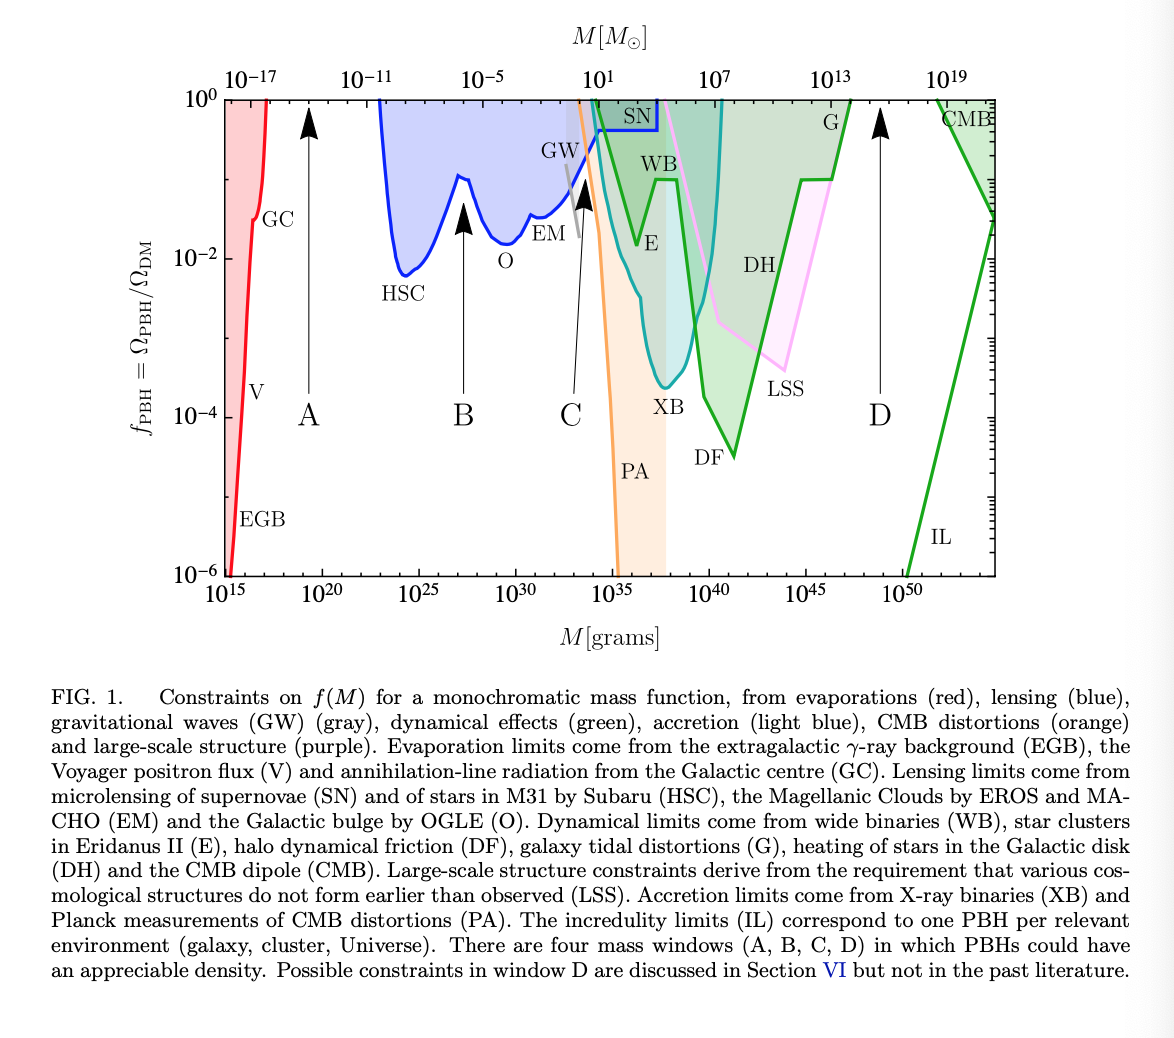
\includegraphics[width=10cm]{Contraints.png}\\
    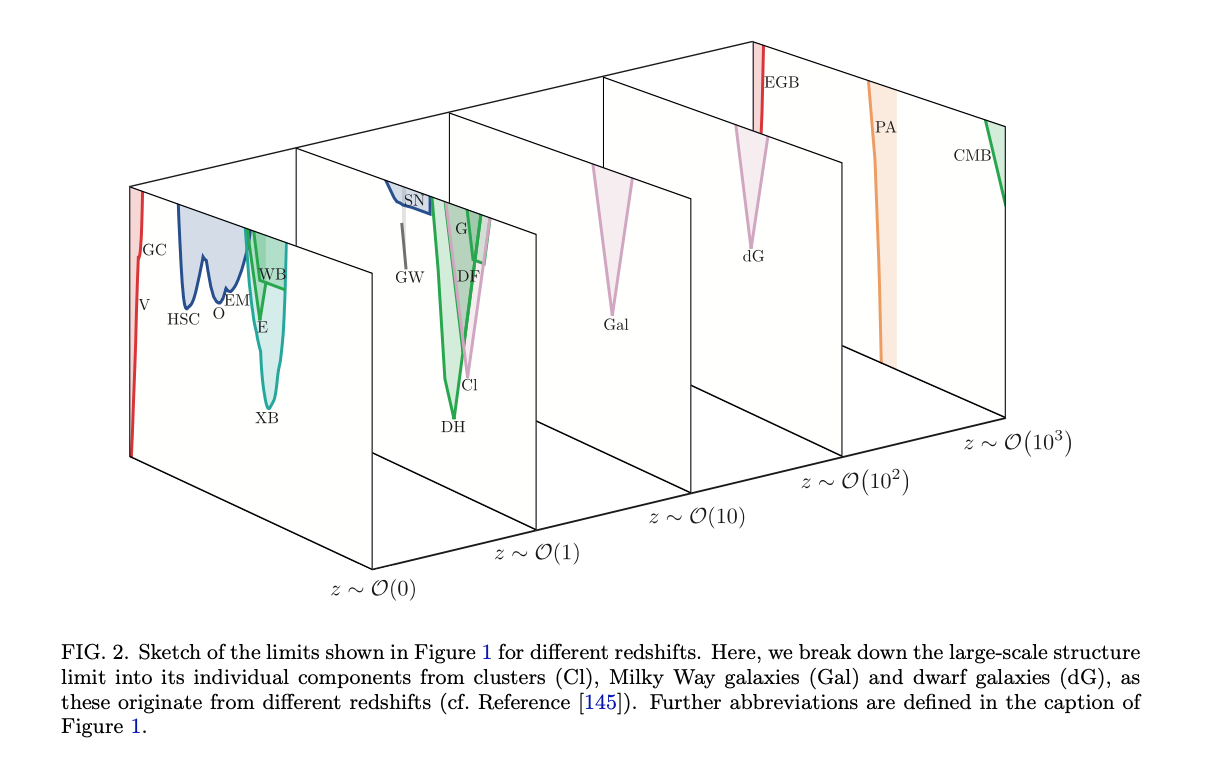
\includegraphics[width=10cm]{ConstraintsWrtRS.png}
    \item So in our RS window, we are pinned btw Voyager positron flux (V) \& annihilation-line radiation from galactic center (GC) and lensing of stars in M31 (HSC) but mostly the former
    \item There is a strong constraint on $f(M_*)$ from observations of the extragalactic $\gamma$-ray background where $M_* \approx 5\times10^14$g is the evaporating mass (Hawking, Gamma rays from primordial black holes)
    \item PBHs in the band $M_* < M < 1.005M_*$ have not yet completed evap but are below $M_q \approx 0.4M_*$ where quark and gluon jets can be emitted (HOW MUCH do JET PHOTONS affect our spectrum? Worth looking into?)
    $$f(M) < 2\times10^{-8}(\frac{M}{M_*})^{3 +\epsilon} \mbox{ for } (M>M_*)$$
    \item Galactic gamma-ray bkg could give stronger limit BUT depends on PBH mass fcn (EGB)
    \item Positron data from Voyager 1 constrains PBHs of $M<10^16$g to $f<0.001$
    \item Gonna skip the rest of the constraints in favor of more relevant stuff
\end{itemize}

\subsection{Evidence for Primordial Black Hole Final Evaporation - Cline '09}
\begin{itemize}
    \item Only survival time of 1s to 1ms would allow for a detectable GRB with existing space detectors (LAT launched in 2008)
    \item Clear asymmetry in VSB locations; local galactic source  -- WHAT COORDS SPECIFICALLY? looks to be RHS octant
    \item I want to figure out Stefano's method for the burst duration, so that we can back-calculate Cline's fascination with roughly 10ms bursts
\end{itemize}

\subsection{Fermi Collaboration Search for GRBs from EBHs (Ritz, Atwood, Omodei)}
Note: Arne Christian Johnson's PhD thesis has some more description of methodology (73, pg 91 in the pdf)
\begin{itemize}
    \item Temperature of 20MeV for EBHs evaporating rn
    \item Distance to which a PBH of 16GeV can be detected is $\leq 0.02$pc
    \item Fermi-LAT is sensitive to a PBH evap rate of $6\times 10^4 pc^{-3} yr^{-1}$\\
    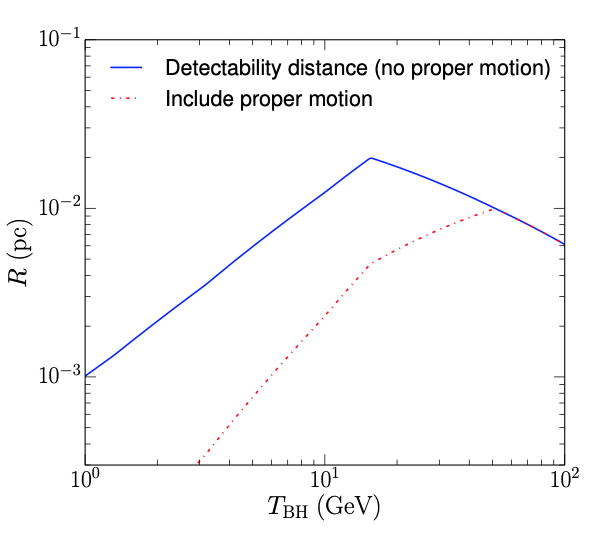
\includegraphics[width=10cm]{FLDetectability.png}
\end{itemize}

\end{document}